\documentclass[]{interact}

\usepackage{epstopdf}
\usepackage[caption=false]{subfig}
\usepackage{amsmath,amssymb,amsthm}
\usepackage{booktabs}

\usepackage[natbibapa]{tfapastyle}
\setlength\bibhang{12pt}
\renewcommand\bibliographytypesize{\fontsize{10}{12}\selectfont}

\usepackage{hyperref}
\usepackage{url}

\theoremstyle{plain}
\newtheorem{theorem}{Theorem}[section]
\newtheorem{lemma}[theorem]{Lemma}
\newtheorem{corollary}[theorem]{Corollary}
\newtheorem{proposition}[theorem]{Proposition}

\theoremstyle{definition}
\newtheorem{definition}[theorem]{Definition}
\newtheorem{example}[theorem]{Example}

\theoremstyle{remark}
\newtheorem{remark}{Remark}
\newtheorem{notation}{Notation}

\begin{document}

\articletype{RESEARCH ARTICLE}

\title{Visual Number Algebras: From Binary XOR-Convolution to Painterly Prime-Factor Superposition}

\author{
\name{Leonardo Ara\'{u}jo\textsuperscript{a}\thanks{CONTACT Leonardo Ara\'{u}jo. Email: leolca@ufsj.edu.br}}
\affil{\textsuperscript{a}DTECH/UFSJ --- Universidade Federal de S\~{a}o Jo\~{a}o del-Rei, Ouro Branco, MG, Brazil}
}

\maketitle

\begin{abstract}
Visual representations of integer factorization—such as side-by-side prime motifs or nested geometric diagrams—typically require knowing a number's prime factors in advance in order to draw it. We investigate a complementary question: can we assign visual patterns to numbers over a finite range $\{1, \dots, N\}$ so that \emph{visual composition itself} mirrors integer multiplication, $\Phi(a \cdot b) = \Phi(a) \star \Phi(b)$, and so that factors can be recovered back from the resulting image? We present two families of solutions. First, we construct an exact pixel-level commutative monoid homomorphism using 2D cyclic XOR-convolution in the finite polynomial ring $\mathbb{F}_2[x,y]/(x^W - 1, y^H - 1)$, showing that $9 \times 9$ odd-weight prime basis tiles yield $120/120$ collision-free binary patterns for $1 \le n \le 120$ while supporting lossless two-tone and geometric presentations (organic ink, diamonds, radial mandalas). Second, we explore three painterly superpositions—inspired by Jackson Pollock's drip paintings, Paul Klee's 1914 watercolors, and Wassily Kandinsky's \emph{Composition VIII}—where each prime factor acts as a deterministic generator of strokes, watercolor glazes, or geometric forms. Across all four systems, we verify $120/120$ image uniqueness and $120/120$ exact blind factor recovery via bitmask matching or occlusion-aware layer peeling.
\end{abstract}

\begin{keywords}
mathematical art; prime factorization; visual algebra; 2D XOR-convolution; generative painting; invertibility
\end{keywords}

\section{Introduction}
Although we encounter positive integers early in life through counting, labeling, and measurement, numbers themselves are abstract entities independent of any single notation \citep{menninger1969number,reimann2024visual}. Societies have historically adopted different positional bases for practical reasons \citep{ifrah2000universal,menninger1969number}: \emph{base 10} (decimal) reflects anatomical finger counting; \emph{base 12} (duodecimal, preserved in dozens and clock faces) offers convenient divisibility by $2, 3, 4$, and $6$; and \emph{base 60} (sexagesimal, inherited from Babylonian astronomy and still used for minutes, seconds, and angular degrees) maximizes small-integer divisors. Yet all positional bases—including binary base $2$—are optimized for addition and magnitude comparison rather than multiplicative structure: in base $10$, consecutive numerals such as $14$ and $15$ conceal that $14 = 2 \times 7$ and $15 = 3 \times 5$.

Representing integers directly through \emph{prime factorization} reveals that hidden structure—fulfilling what \citet{arcavi2003role} describes as visualization's role in ``seeing the unseen'' within abstract mathematical objects, and echoing \citet{harriss2022art} in viewing mathematical illustration as an inherently artistic mapping from abstract structure into perceptual form. By the \emph{Fundamental Theorem of Arithmetic}, every integer $n > 1$ admits a decomposition into prime numbers that is unique up to the ordering of factors:
\[
  n = \prod_{i=1}^{r} p_i^{e_i},
\]
where $p_1 < p_2 < \dots < p_r$ are distinct primes and $e_i \ge 1$ are their multiplicities (with $n = 1$ serving as the empty product, or multiplicative identity). Integer factorization and the Fundamental Theorem of Arithmetic have long been of central interest across mathematics, computer science, and engineering—from pure number theory to cryptography and error-correcting codes—because multiplication is computationally easy while recovering prime factors is hard. In this paper, we draw a parallel into the visual art world: if each prime is assigned an irreducible visual motif, how can we compose them so that visual combination mirrors multiplication and every composite inherits a unique, recoverable artistic signature?

Visual symbols have long been used to encode structured information—from maritime signal flags and Morse code's dots and dashes to the bars of linear barcodes and the pixel matrices of QR codes. While these modern codes are engineered for efficiency and unambiguous decoding, they rarely aspire to aesthetic beauty. Yet history and literature offer striking counterexamples where information encoding and visual art are inseparable: Egyptian hieroglyphs, East Asian kanji calligraphy, and—in a playful cryptographic vein—Arthur Conan Doyle's \emph{The Adventure of the Dancing Men}, where stick-figure postures serve simultaneously as a substitution cipher and a decorative frieze. In the philosophy of art, \citet{goodman1968languages} formalizes this capacity by showing that pictures and notations operate as \emph{symbol systems} governed by syntactic and semantic rules rather than mere resemblance—an insight that aligns naturally with discrete, differentiable computational tokens. Standing at the intersection of mathematics and the arts \citep{emmer1993visual}—and echoing the program of \emph{aesthetic computing} \citep{fishwick2006aesthetic}, which brings artistic theory and culturally specific styles (such as the Bauhaus school) into formal \emph{notational spaces}—we aim for this same duality: visual number representations that are simultaneously \emph{efficiently composable and recoverable} like a mathematical code, yet \emph{aesthetically compelling} as visual art.

In \emph{Prime concerns: painting number patterns}, \citet{ashwell2020prime} assigns distinct visual marks to prime numbers and depicts composite numbers by placing those marks side by side. Related visual traditions—including Huff's 3D ``genetic'' prime-factor sculptures \citep{huff2006visually}, Yorgey's recursive \emph{Factorization Diagrams} \citep{yorgey2012factorization}, Reimann's geometric integer patterns \citep{reimann2024visual}, the color-segmented wheels of \emph{Prime Climb}, and Ba\c{s}e\u{g}mez's dihedral rosette pictographs \citep{basegmez2026symmetries}—share a common workflow: one first factors $n$ arithmetically and then arranges symbols according to that factorization. In computational neuroscience, \citet{kleyko2022integer} take a complementary algebraic step using Vector Symbolic Architectures, binding prime hypervectors so that multiplication becomes compositional binding and factorization becomes resonator-network unbinding.

Here we ask whether the visual representation can instead carry an \emph{internal composition law} $\star$ such that combining the images of $a$ and $b$ directly produces the image of $a \cdot b$, without re-factoring:
\begin{equation}
  \Phi(a \cdot b) = \Phi(a) \star \Phi(b), \qquad a, b \in \{1, \dots, N\}.
\end{equation}
A naive attempt using pixelwise binary XOR ($\oplus$) fails on prime powers because $x \oplus x = 0$, causing $4 = 2^2$ to collapse to the blank tile and $8 = 2^3$ to revert to $2$. On the other hand, hashing $(p, e, r, c)$ per pixel avoids cancellation but breaks the visual composition law: $\Phi(4)$ can no longer be formed from $\Phi(2)$ and $\Phi(2)$ alone.

To resolve this tension, we develop and compare two complementary approaches over the range $1 \le n \le 120$:
\begin{enumerate}
  \item \textbf{An exact binary algebra} based on 2D cyclic XOR-convolution in $\mathbb{F}_2[x,y]/(x^9 - 1, y^9 - 1)$, paired with lossless artistic presentations that remain $100\%$ convertible back to $0/1$ matrices.
  \item \textbf{Three painterly superpositions} inspired by Jackson Pollock, Paul Klee (1914), and Wassily Kandinsky (\emph{Composition VIII}, 1923), where multiplication corresponds to superimposing or glazing prime-seeded visual gestures.
\end{enumerate}

\section{Exact Visual Algebra via 2D Cyclic XOR-Convolution}
Let $R_{W,H} = \mathbb{F}_2[x, y] / (x^W - 1, y^H - 1)$ be the quotient polynomial ring of binary $W \times H$ tiles over the finite field $\mathbb{F}_2$ \citep{lidl1997finite,dummit2003abstract}, where each tile $A \in \{0,1\}^{H \times W}$ is identified with the polynomial
\[
  A(x,y) = \sum_{r=0}^{H-1} \sum_{c=0}^{W-1} A_{r,c}\, x^c y^r \in R_{W,H}.
\]
Multiplication in $R_{W,H}$ is \emph{2D cyclic XOR-convolution} (closely related to the polynomial representation of linear cellular automata over $\mathbb{F}_2$ studied by \citet{martin1984algebraic}):
\begin{equation}
  (A \star B)_{r,c} = \bigoplus_{i=0}^{H-1} \bigoplus_{j=0}^{W-1} A_{i,j} \cdot B_{(r-i)\bmod H,\; (c-j)\bmod W}.
\end{equation}
The single-pixel tile $I_{0,0} = 1$ serves as the multiplicative identity $\Phi(1) = 1$, and $\star$ is commutative and associative by ring structure.

\begin{proposition}[Preservation of Prime Powers]
In characteristic $2$, squaring any tile $A(x,y) \in R_{W,H}$ satisfies
\[
  A(x,y)^2 = A(x^2, y^2) \pmod{(x^W - 1, y^H - 1)}.
\]
When $W$ and $H$ are odd, $z \mapsto 2z \bmod W$ is a permutation of $\{0,\dots,W-1\}$, so squaring acts as a toroidal geometric dilation rather than collapsing $A$ to zero.
\end{proposition}

To avoid evaluating to zero at $(x,y) = (1,1)$ (which occurs whenever a tile has an even number of lit bits), we restrict prime basis tiles to odd Hamming weight ($k \in \{3, 5\}$). Using a greedy incremental search in $R_{9,9}$, we obtain a prime basis for all $30$ primes $\le 120$ such that every $n \in \{1,\dots,120\}$ maps to a unique $9 \times 9$ binary tile (Figure~\ref{fig:xor_grid}), with bit densities ranging from $1.2\%$ ($\Phi(1)$) to $50.6\%$ (median $11.1\%$).

\begin{figure}[t]
  \centering
  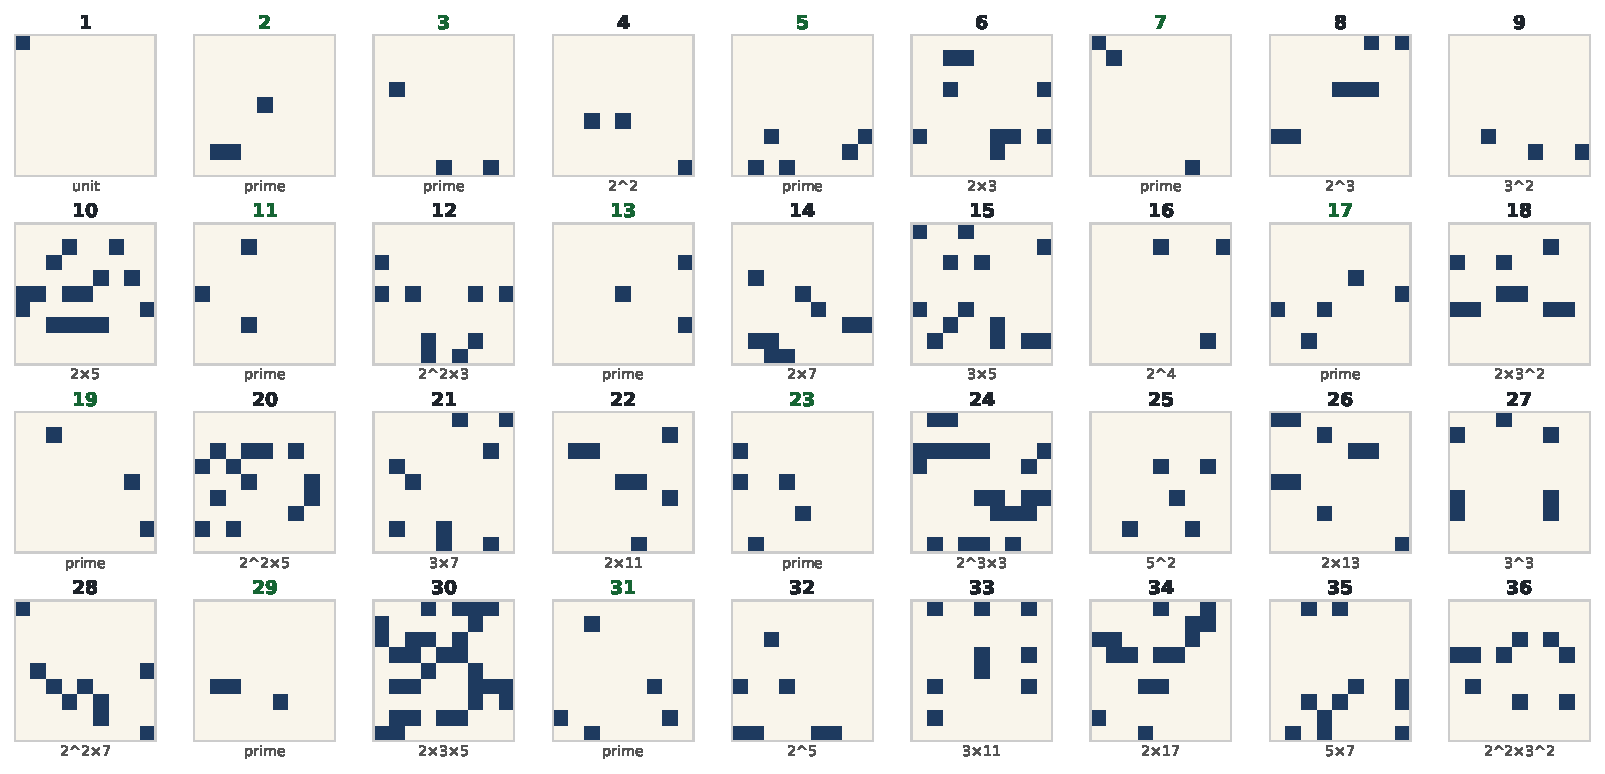
\includegraphics[width=\textwidth]{figures/fig1_xor_grid.pdf}
  \caption{The first $36$ tiles generated by 2D cyclic XOR-convolution in $\mathbb{F}_2[x,y]/(x^9-1, y^9-1)$. Every integer $n \in \{1,\dots,120\}$ receives a unique binary pattern while satisfying $\Phi(a\cdot b) = \Phi(a) \star \Phi(b)$.}
  \label{fig:xor_grid}
\end{figure}

\subsection{Lossless Presentation Decoupling and Binary Generative Grammar}
While raw black-and-white pixels make the algebra explicit, any bijective rendering of the $0/1$ grid preserves exact recoverability—realizing the content--presentation separation advocated in aesthetic computing \citep{fishwick2006aesthetic}. Figure~\ref{fig:xor_presentations} illustrates four lossless renderings of $\Phi(30) = \Phi(6) \star \Phi(5)$: raw binary, connected organic ink (fusing orthogonally adjacent `1` cells), rotated diamonds, and a radial mandala mapping $(r,c)$ to concentric rings and angular sectors. Sampling cell centers (or thresholding the two-tone palette) recovers the exact underlying matrix in $R_{9,9}$.

For direct comparison with the painterly systems below, we also construct a \emph{bitwise OR generative grammar} over $9 \times 9$ binary tiles: each prime $p$ receives a connected $3$- to $4$-bit polyomino block motif $G_{p,1}$, each higher exponent $e \ge 2$ adds a $2$- to $3$-bit domino or corner block ($G_{p,1} \subset G_{p,2} \subset \dots$), and composites take the bitwise union $\bigvee_i G_{p_i, e_i}$. Unlike XOR-convolution, this preserves every prime's visible block motif intact inside composites (like radicals in kanji), while remaining $120/120$ unique and blindly recoverable via subset-pruned search.

\begin{figure}[t]
  \centering
  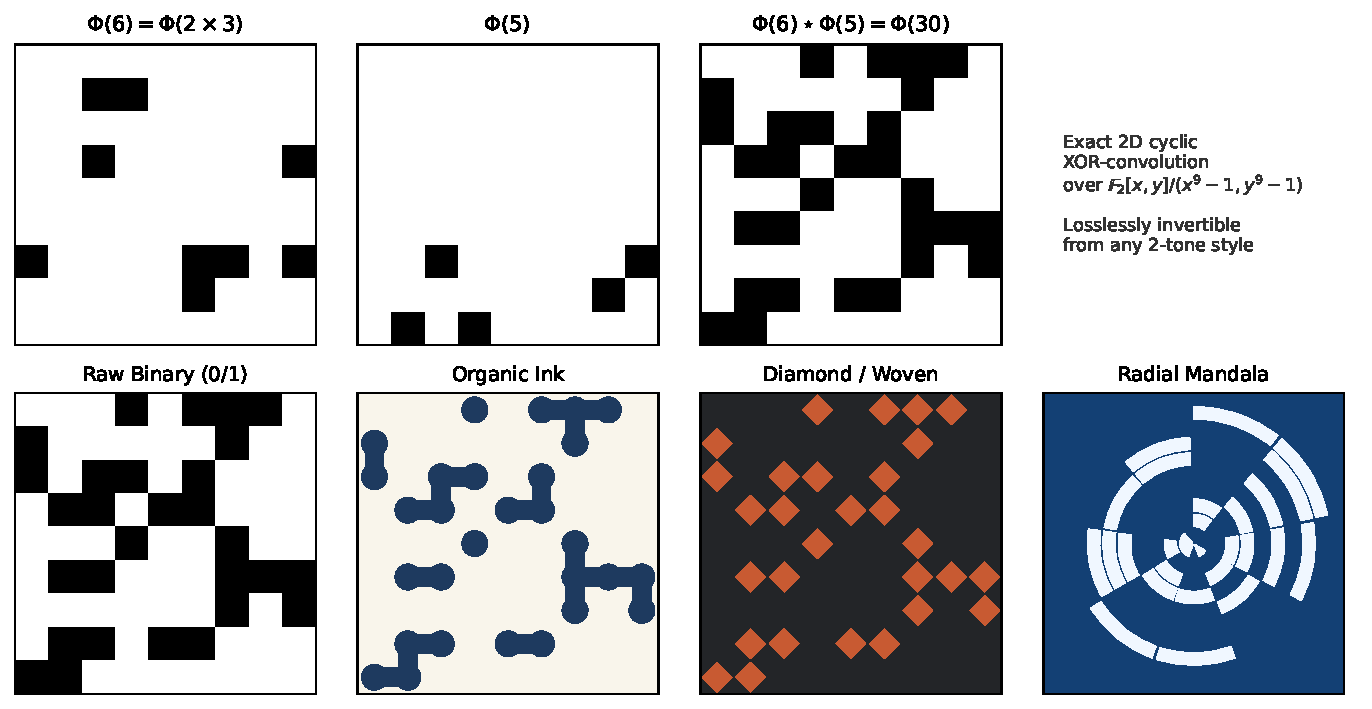
\includegraphics[width=0.95\textwidth]{figures/fig2_xor_presentations.pdf}
  \caption{Top: direct composition $\Phi(6) \star \Phi(5) = \Phi(30)$ in $R_{9,9}$. Bottom: four lossless two-tone and geometric presentations of the same binary matrix $\Phi(30)$.}
  \label{fig:xor_presentations}
\end{figure}

\section{Artistic Precedents and Stylistic Grammars}
To bridge arithmetic structure with recognizable visual traditions, our painterly systems draw on three twentieth-century masters whose formal vocabularies map naturally onto prime-factor decomposition:

\begin{itemize}
  \item \textbf{Jackson Pollock (Drip Painting, c.\ 1947--1950).}
  Pollock's "all-over" drip canvases abandon a single focal center in favor of interwoven trajectories of poured paint, where rapid wrist flicks leave thin filaments and pauses pool into droplets and splatters. In our arithmetic translation, each prime factor initiates an independent gestural trajectory in its own hue. Encoding exponent $e$ as trajectory extent turns prime powers ($2, 4, 8, \dots$) into temporally extended gestures along a shared path, while composites interleave multiple colored trajectories across the same canvas.

  \item \textbf{Paul Klee (1914 Watercolors).}
  During and immediately after his 1914 trip to Tunisia, Klee developed luminous watercolor compositions built from translucent rectangular bands, alternating horizontal and vertical rhythms, and overlapping pigment glazes where intersecting washes produce secondary tones. Translating each prime into a translucent watercolor band whose orientation alternates by prime index causes composite numbers (such as $6 = 2 \times 3$) to form perpendicular grid intersections, while edge wrap-around with stroke-width spacing turns higher exponents into rhythmic multi-band progressions.

  \item \textbf{Wassily Kandinsky (\emph{Composition VIII}, 1923).}
  Painted during his Bauhaus period, Kandinsky's \emph{Composition VIII} exemplifies a geometric-abstract grammar built from circles, concentric rings, acute triangles, semicircles, parallelograms, checkerboards, and parallel line bundles with crossbar ticks, suspended on a warm parchment ground. Because each prime requires a distinct visual identity, this rich geometric taxonomy accommodates dozens of primes cleanly; low-discrepancy spatial placement preserves Kandinsky's balanced distribution of anchors and accents, while multiplicity varies scale, pigment, and filled-versus-outlined rendering.
\end{itemize}

\section{Painterly Superpositions}
To explore richer color and compositional structure, we also investigate three generative painting systems where each prime $p$ seeds a deterministic pseudorandom generator (\texttt{mulberry32}):
\begin{itemize}
  \item \textbf{Pollock Drip-Paths:} Each prime $p$ is assigned a hue via golden-angle spacing ($137.508^\circ$) and traces a momentum-driven quadratic B\'ezier trajectory with velocity-coupled stroke width and splatter droplets. Multiplicity $p^e$ can be encoded as $e$ separate strokes, as \emph{path extent} ($S \cdot e$ steps along the same trajectory, giving prime powers $p^1 \subset p^2 \subset p^3$ a prefix-preserving visual lineage), or in two true homomorphism variants: \emph{translucent \texttt{multiply} coats} ($A_p^e$, yielding a pixel-level homomorphism for all $a,b$) and \emph{toroidal Fourier trajectory addition} ($\gamma_n(t) \equiv \sum_i e_i \gamma_{p_i}(t) \pmod{1}$ on $[0,1)^2$, yielding a vector-space homomorphism $\gamma_{a\cdot b} \equiv \gamma_a + \gamma_b$).
  \item \textbf{Klee 1914 Watercolor:} Inspired by Paul Klee's 1914 watercolors, each prime paints a translucent \texttt{multiply}-blended band whose orientation alternates between horizontal and vertical by prime index, whose length scales with $e$, and which wraps across canvas edges by jumping a spacing proportional to its stroke width.
  \item \textbf{Kandinsky \emph{Composition VIII}:} Each prime $p$ is assigned a geometric form (circle, triangle, parallel line bundle, semicircle, rectangle, lozenge, square, parallelogram, hexagon, heptagon, double ring, or $3\times 3$ checkerboard) and placed via a low-discrepancy 2D Halton sequence indexed strictly by $(p, k)$ so that primes retain their exact positions in all composites. Repeated occurrences $k=1,\dots,e$ vary in scale, fill/outline style, and pigment.
\end{itemize}
Figure~\ref{fig:gallery} compares all three painterly modes across two rows of prime powers and composites ($2, 4, 8, 6, 12, 30$ and $32, 36, 60, 96, 105, 120$).

\subsection{Homomorphism vs.\ Generative Grammar}
The systems explored in this paper highlight a fundamental design spectrum between \emph{true visual homomorphisms} and \emph{factor-driven generative grammars}:

\begin{itemize}
  \item \textbf{True Visual Homomorphisms ($\Phi(a \cdot b) = \Phi(a) \star \Phi(b)$).}
  In 2D cyclic XOR-convolution, Pollock Translucent Multiply, and Pollock Trajectory Vector Sum, composition operates directly on the visual representations of $a$ and $b$ without factoring either number.
  \emph{Pros:} algebraic closure, factor-blind composition, exact commutativity ($\Phi(a) \star \Phi(b) = \Phi(b) \star \Phi(a)$), and a direct structural parallel to the multiplicative monoid $(\mathbb{N}^+, \times)$.
  \emph{Cons:} the visual medium must support a non-idempotent, commutative combining law, which restricts the aesthetics to periodic binary grids (XOR), monotonically darkening glazes (\texttt{multiply}), or summed trajectories where individual prime colors merge.

  \item \textbf{Factor-Driven Generative Grammars.}
  In opaque \texttt{source-over} Pollock, extent-wrapped Klee (for shared factors), and Kandinsky \emph{Composition VIII}, the artwork is synthesized from the prime-factor multiset $\{p_i^{e_i}\}$ rather than from flat pixel arrays.
  \emph{Pros:} unrestricted painterly expressiveness—opaque pigments, crisp outlines, balanced spatial layouts, and immediately legible distinct prime motifs.
  \emph{Cons:} flat RGB images cannot generally be combined pixelwise when $\gcd(a,b) > 1$ (e.g., extending a stroke or spawning a new figure) or when opaque layers cross in different orders; composition requires operating at the generator/layer level rather than the flat-pixel level.
\end{itemize}

Table~\ref{tab:proscons} summarizes these trade-offs. Notably, \emph{lossless presentation decoupling} (Section~2.1) and \emph{translucent \texttt{multiply} glazing} bridge both worlds: the former hides an exact binary homomorphism behind organic or geometric styles, while the latter brings pixel-level homomorphism to painterly strokes. From a semiotic perspective, this also explains why human writing systems—such as kanji radicals and Egyptian hieroglyphic quadrats—evolved as generative grammars whose parts remain visually recognizable, whereas machine-oriented encodings such as QR codes rely on finite-field arithmetic ($\mathbb{F}_{2^8}$) that prioritizes algebraic closure over human legibility.

\begin{table}[ht]
  \centering
  \caption{Comparison of true visual homomorphisms and factor-driven generative grammars.}
  \label{tab:proscons}
  \small
  \begin{tabular}{@{}p{3.0cm}p{5.1cm}p{5.1cm}@{}}
    \toprule
    Criterion & Visual Homomorphism & Generative Grammar \\
    \midrule
    Composition law & Factor-blind ($\Phi(a) \star \Phi(b)$) & Requires prime multiset $\{p_i^{e_i}\}$ \\
    Commutativity & Exact by construction & Requires canonical draw order \\
    Prime powers ($p^e$) & Ring dilation, $e$ glazes, or $e\gamma_p$ & New strokes, band length, or echoes \\
    Visual freedom & Constrained by algebra of $\star$ & High (opaque, geometric, spatial) \\
    Blind recovery & Basis search or glaze peeling & Top-down occlusion peeling \\
    \bottomrule
  \end{tabular}
\end{table}

\begin{figure}[t]
  \centering
  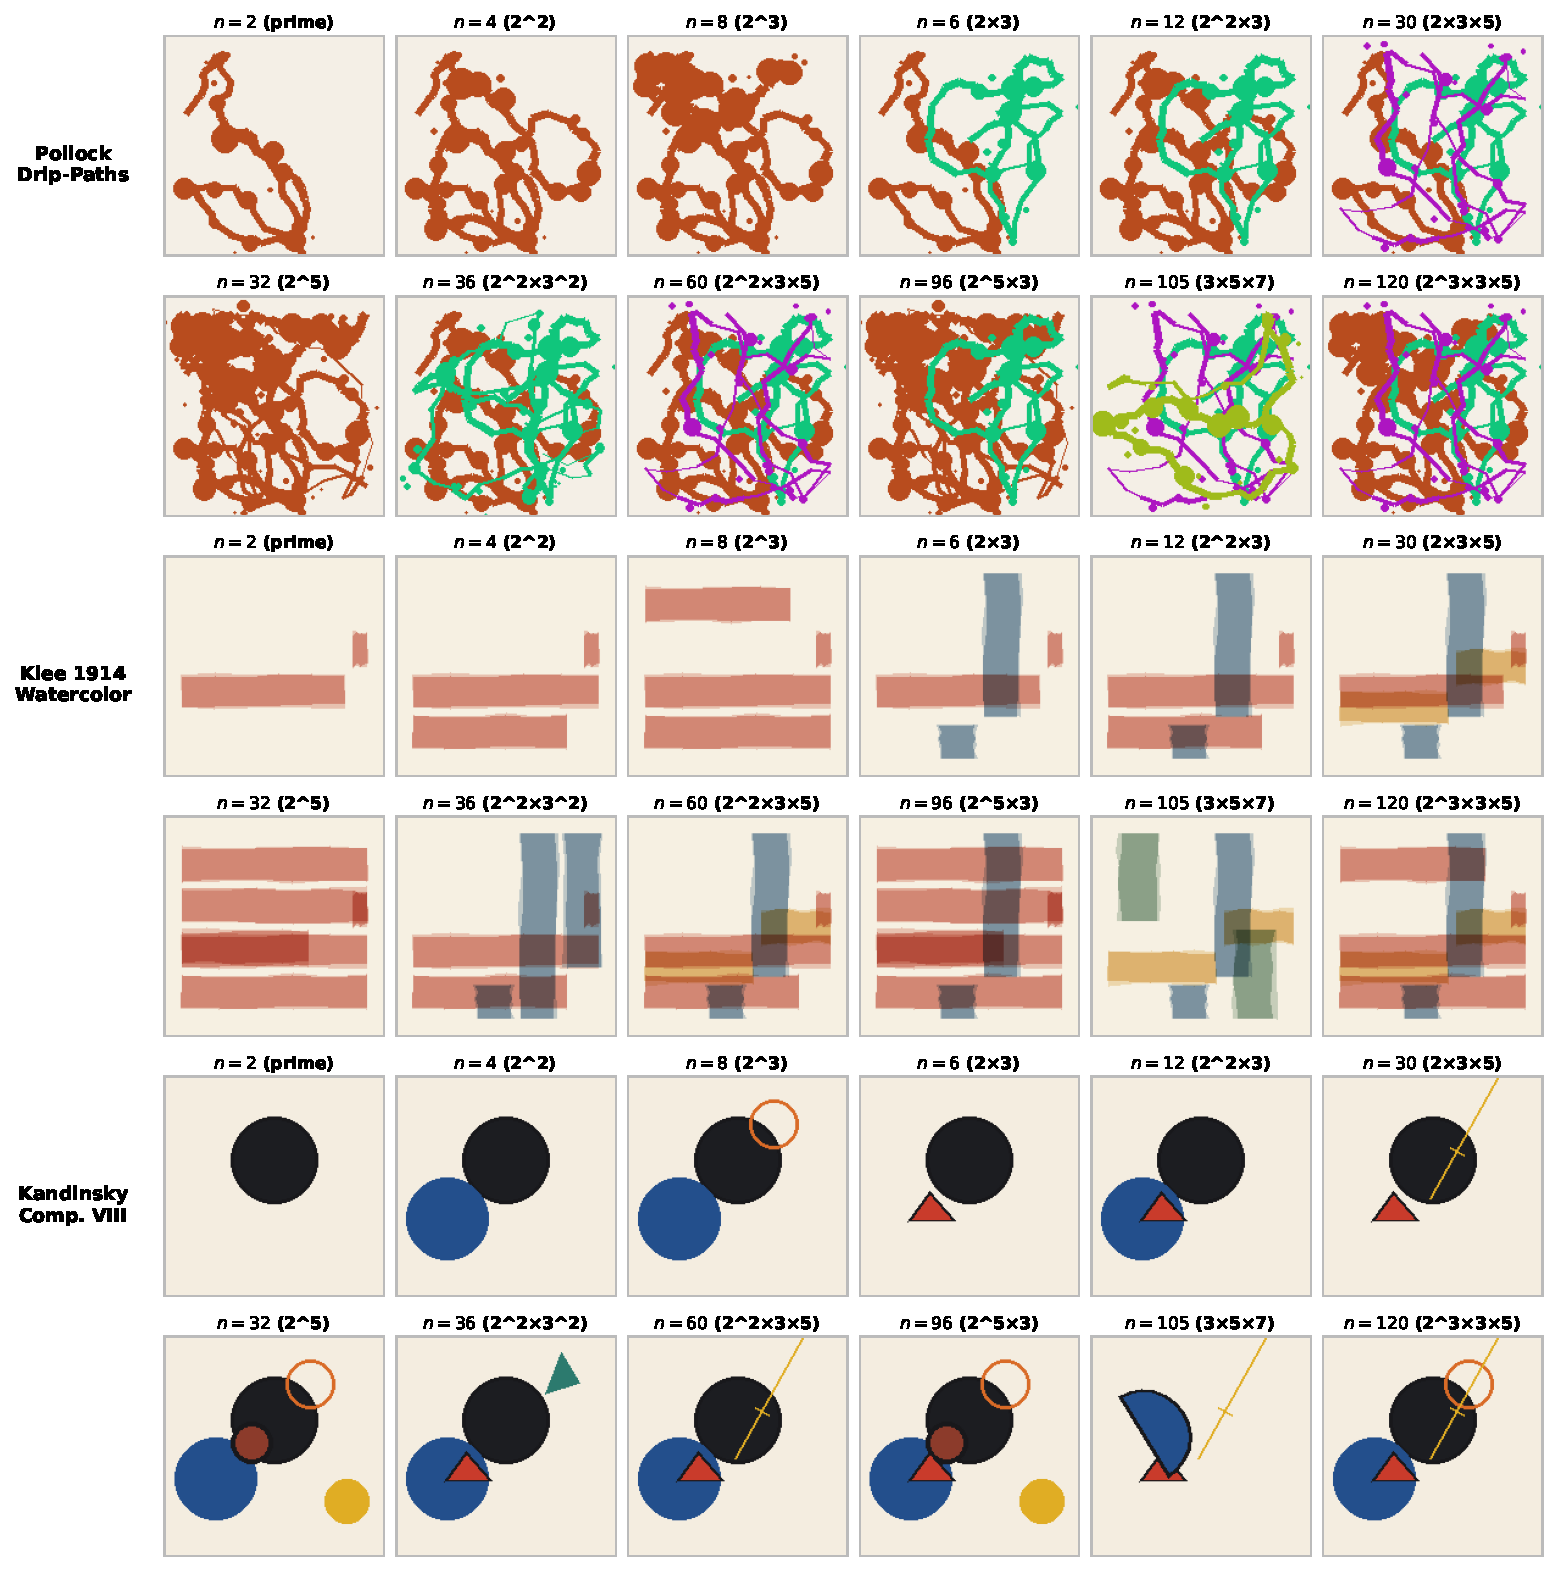
\includegraphics[width=0.98\textwidth]{figures/fig3_painterly_gallery.pdf}
  \caption{Comparison of the three painterly modes across two rows per style: $n \in \{2, 4, 8, 6, 12, 30\}$ and $n \in \{32, 36, 60, 96, 105, 120\}$.}
  \label{fig:gallery}
\end{figure}

\section{Invertibility and Blind Factor Recovery}
A central question for any visual number representation is whether an algorithm can recover $n$ and its prime factorization from an unlabeled image $I$ alone, without access to metadata or a precomputed table of composites. Because our four systems combine factors through fundamentally different mechanisms, each admits a distinct blind recovery procedure:

\begin{enumerate}
  \item \textbf{Prime-Basis Search (2D XOR-Convolution).}
  Given any lossless two-tone or geometric rendering, sampling cell centers (or thresholding the two-color palette) recovers the exact binary matrix $M \in R_{9,9}$. Unlike painterly layers, toroidal XOR-convolution mixes bits globally across the $9 \times 9$ grid, so individual prime footprints cannot be peeled locally. Moreover, odd-weight prime polynomials can act as units in the cyclic ring $R_{9,9}$, meaning ring division $M \cdot P_p^{-1}$ is always defined and does not isolate divisors (in contrast to unwrapped multiplication in $\mathbb{F}_2[x,y]$, which is a unique factorization domain). Instead, given only the $30$ prime basis tiles $\{P_p\}_{p \le 120}$ and the identity $I_{0,0}$, a depth-first search over non-decreasing prime products $\prod p_i^{e_i} \le 120$ incrementally convolves prime tiles until matching $M$, recovering the exact factorization without storing any composite tiles.

  \item \textbf{Top-Down Occlusion-Aware Layer Peeling (Pollock and Kandinsky).}
  In both Pollock and Kandinsky modes, prime occurrences $(p, k)$ are painted in ascending lexicographic order via \texttt{source-over} compositing. Consequently, the largest $(p, k)$ present in a composition is guaranteed to be \emph{completely unoccluded}. Let $\mathcal{O} \subseteq \{1,\dots,S\}^2$ denote the set of pixels already accounted for by peeled layers (initially $\mathcal{O} = \emptyset$). Iterating candidate templates $(p, k)$ in descending order, we inspect the unoccluded footprint $U_{p,k} = \operatorname{supp}(T_{p,k}) \setminus \mathcal{O}$. Whenever $U_{p,k} \neq \emptyset$ and $I$ matches $T_{p,k}$ on $U_{p,k}$, we record $(p, k)$ and update $\mathcal{O} \leftarrow \mathcal{O} \cup \operatorname{supp}(T_{p,k})$ before testing smaller primes (Figure~\ref{fig:peeling}).

  \item \textbf{Multiplicative Glaze Peeling (Klee 1914 Watercolor).}
  In Klee mode, translucent bands combine via \texttt{multiply} blending rather than opaque occlusion. Each prime-power band $(p, e)$ multiplies the normalized paper ground $R = I / I_{\mathrm{bg}} \in (0, 1]^3$ by a per-pixel attenuation field $A_{p,e} \in (0, 1]^3$ (equal to $1$ outside the band). Because \texttt{multiply} blending only darkens pixels, any band $(p, e)$ present in $I$ must satisfy $R(x,y) \le A_{p,e}(x,y) + \varepsilon$ across its entire support (where $\varepsilon = 0.015$ absorbs 8-bit quantization). Iterating primes $p$ in descending order and exponents $e$ from $\lfloor \log_p N \rfloor$ down to $1$, whenever this inequality holds we record $p^e$ and divide out the glaze: $R \leftarrow \min(1, R / A_{p,e})$.
\end{enumerate}

\begin{figure}[t]
  \centering
  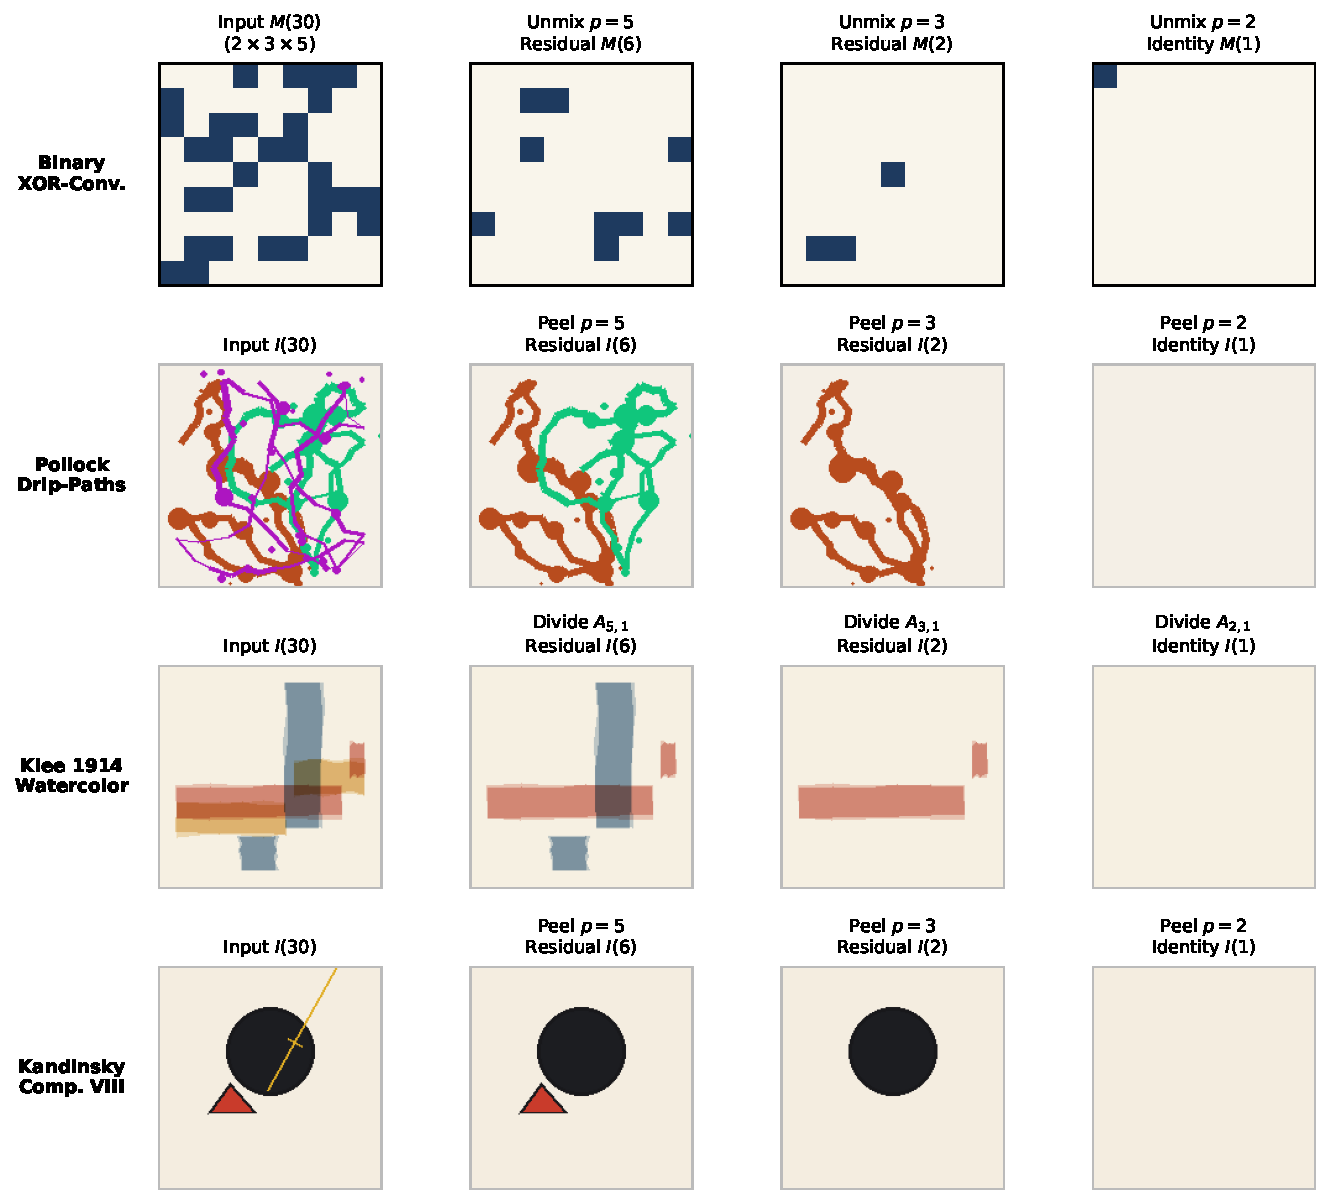
\includegraphics[width=0.95\textwidth]{figures/fig4_peeling_decomposition.pdf}
  \caption{Step-by-step blind factor recovery of $n = 30 = 2 \times 3 \times 5$ across all four systems: prime-basis unmixing for Binary XOR-Convolution, top-down layer peeling for Pollock and Kandinsky, and multiplicative glaze division for Klee 1914 Watercolor.}
  \label{fig:peeling}
\end{figure}

Table~\ref{tab:verification} summarizes our empirical verification across all $n \in \{1, \dots, 120\}$ on $100 \times 100$ lossless renders: all seven variants achieve $120/120$ unique images and $120/120$ exact blind factor recovery ($0$ errors), and the three homomorphism modes exhibit $0$ homomorphism errors across all $a \cdot b \le 120$.

\begin{table}[ht]
  \centering
  \caption{Empirical uniqueness, blind factor recovery, and homomorphism checks across $n = 1 \dots 120$.}
  \label{tab:verification}
  \small
  \begin{tabular}{@{}lccc@{}}
    \toprule
    Visual System & Unique Images & Exact Recovery & Hom.\ Errors \\
    \midrule
    1a. Binary XOR-Convolution ($9 \times 9$) & $120 / 120$ & $120 / 120$ & $0$ \\
    1b. Binary OR-Grammar ($9 \times 9$) & $120 / 120$ & $120 / 120$ & --- \\
    2a. Pollock Drip-Paths (opaque, $100^2$) & $120 / 120$ & $120 / 120$ & --- \\
    2b. Pollock Translucent Multiply ($100^2$) & $120 / 120$ & $120 / 120$ & $0$ (pixel) \\
    2c. Pollock Trajectory Vector Sum ($100^2$) & $120 / 120$ & $120 / 120$ & $0$ (vector) \\
    3. Klee 1914 Watercolor ($100^2$) & $120 / 120$ & $120 / 120$ & --- \\
    4. Kandinsky \emph{Comp.\ VIII} ($100^2$) & $120 / 120$ & $120 / 120$ & --- \\
    \bottomrule
  \end{tabular}
\end{table}

\section{Scaling, Capacity, and Message Encoding}
A natural question is how far $N$ can be increased to store more bits per image, and how these representations behave when encoding arbitrary digital messages:

\begin{itemize}
  \item \textbf{Capacity limits per system.}
  In $R_{W,H} = \mathbb{F}_2[x,y]/(x^W-1, y^H-1)$, capacity is bounded by $W \times H$ bits, and avoiding cyclic wrap-around of powers of $2$ requires $\operatorname{lcm}(\operatorname{ord}_W(2), \operatorname{ord}_H(2)) > \lfloor \log_2 N \rfloor$ (e.g., $W=H=9$ suffices up to $2^{63}$, while $W=H=11$ suffices up to $2^{1023}$). In practice, $N=256$ ($8$ bits/tile) or $N=1024$ ($10$ bits/tile) is fast on $11 \times 11$ or $13 \times 13$ grids. For the painterly modes, capacity is bounded by 8-bit color saturation under repeated \texttt{multiply} coats ($\approx 8$--$10$ coats) and by visual clutter as the number of prime factors $\Omega(n) \le \lfloor \log_2 N \rfloor$ grows.

  \item \textbf{Chunked message encoding.}
  Rather than forcing a single tile to represent a huge integer, arbitrary byte streams can be split into fixed-range symbols (just as QR codes split data into finite-field symbols): mapping each byte $b \in \{0,\dots,255\}$ to $n = b + 1 \in \{1,\dots,256\}$ (or using $N=120$ for printable ASCII) allows any message to be rendered as a frieze or mosaic of artistic tiles. Figure~\ref{fig:leonardo} illustrates the 8-character word \texttt{"MathArts"} (ASCII codes $77, 97, 116, 104, 65, 114, 116, 115$, all within $N=120$) encoded across Organic Ink XOR-convolution, Pollock drip-paths, Klee watercolor, and Kandinsky \emph{Composition VIII}.

  \item \textbf{Scope and robustness.}
  Although unbounded trajectory sums are hard to invert from a static bitmap once self-intersections accumulate, the underlying map $\mathbf{e} \mapsto \gamma_n$ is linear in the exponent vector and thus serves as an \emph{artistic watermark or visual code} rather than a cryptographic primitive. Likewise, our current blind decoders operate on lossless, pixel-aligned bitmaps; extending them to photographed or print-and-scan artworks requires adding corner fiducial markers for geometric registration and soft correlation thresholds for quantization noise.
\end{itemize}

\begin{figure}[t]
  \centering
  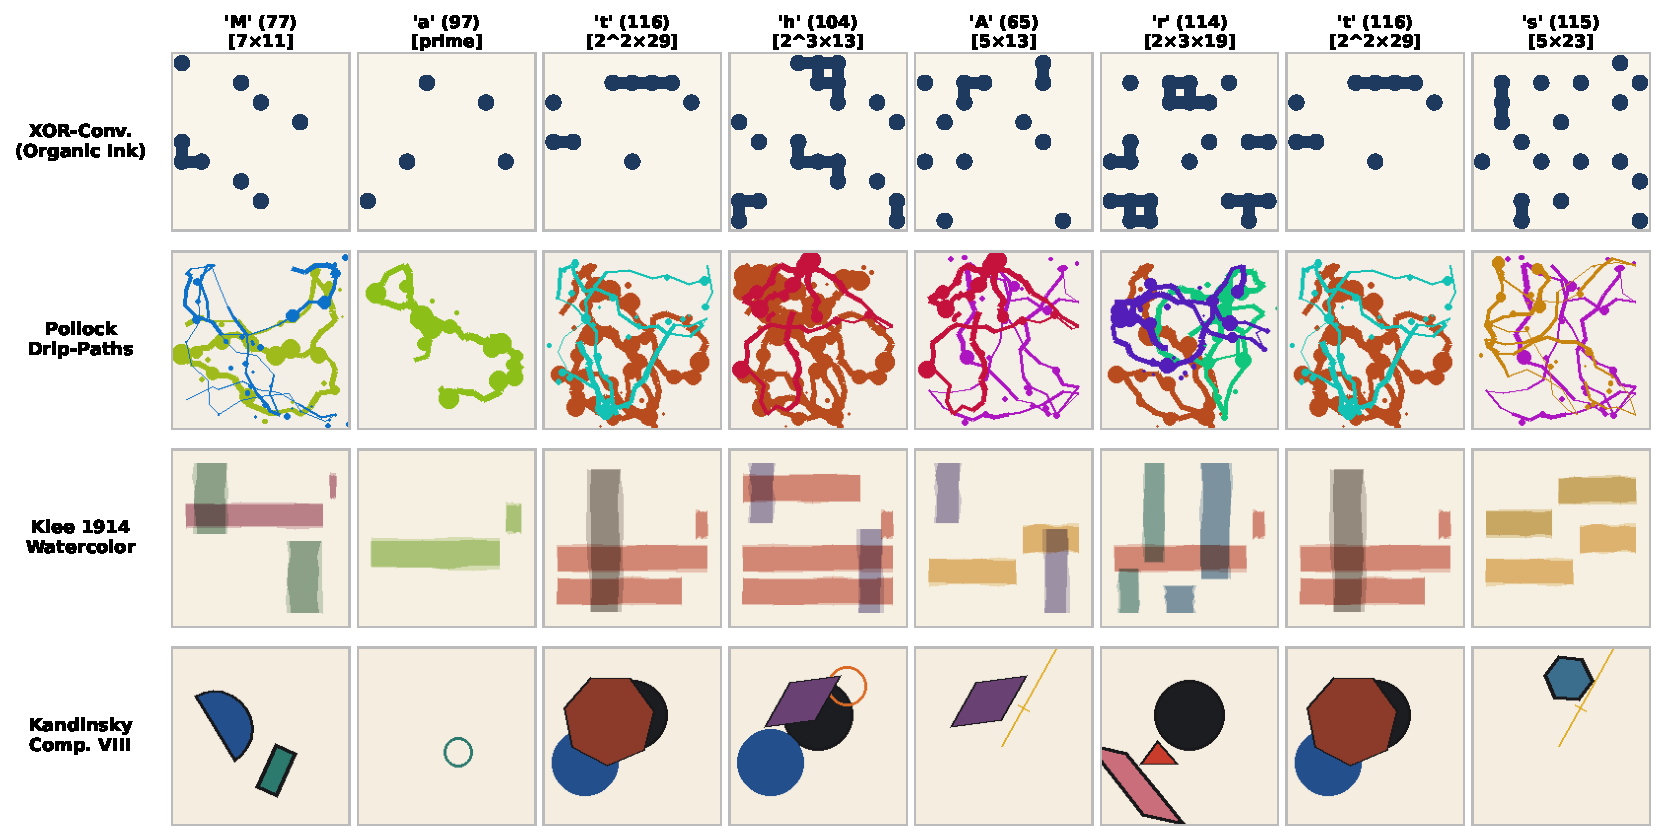
\includegraphics[width=\textwidth]{figures/fig5_message_matharts.pdf}
  \caption{Encoding the 8-character string \texttt{"MathArts"} (ASCII $77, 97, 116, 104, 65, 114, 116, 115$) as an 8-tile artistic frieze under Binary XOR-Convolution (Organic Ink), Pollock Drip-Paths, Klee 1914 Watercolor, and Kandinsky \emph{Composition VIII}.}
  \label{fig:leonardo}
\end{figure}

\subsection{Single-Canvas Pollock Encoding and RTS/Noise Resilience}
As an extension of the Pollock \texttt{multiply} model, an entire $K$-bit string can also be encoded onto \emph{one unified $512 \times 512$ canvas} by mapping bit $i$ to prime $p_i$ (e.g., primes $2 \dots 311$ for $64$-bit \texttt{"MathArts"}, or $2 \dots 719$ for $128$ bits) and integrating an opaque crimson Pollock top-skein ($T_0$) for Fourier--Mellin (log-polar FFT) registration, paired with a log-attenuation linear solver $L_{\mathrm{obs}} = -\log(I/I_{\mathrm{bg}}) \approx \sum b_i L_i$. Across a $100$-trial Monte Carlo benchmark of random $128$-bit messages ($12{,}800$ bits per regime), this single-canvas codec achieves $100/100$ exact messages ($100.00\%$ bits) on clean canvases, $86/100$ exact messages ($99.69\%$ bits) under random rotation/translation/scaling (RTS) + JPEG ($q=80$), and $86/100$ exact messages ($99.72\%$ bits) under random RTS + additive Gaussian noise ($\sigma=8$), while recovering \texttt{"MathArts"} with $64/64$ exact bits in all tested regimes (Figure~\ref{fig:report_rts}).

\begin{figure}[t]
  \centering
  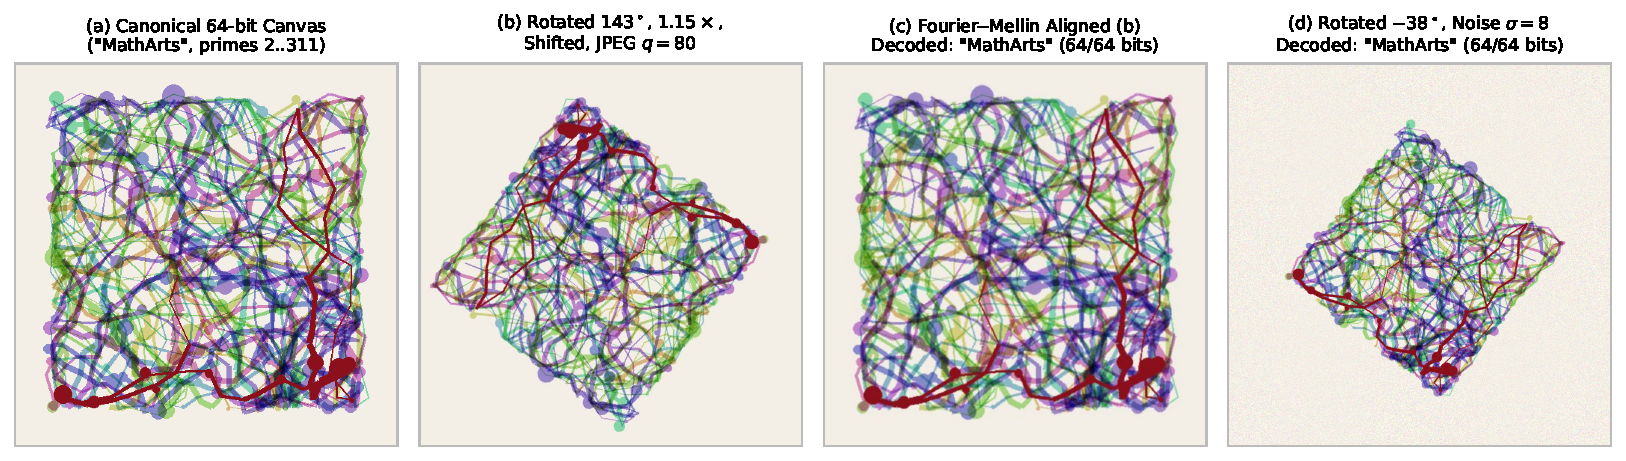
\includegraphics[width=\textwidth]{figures/fig4_pollock_matharts_rts.pdf}
  \caption{Single-canvas $64$-bit encoding of \texttt{"MathArts"} (primes $2 \dots 311$, $512 \times 512$, organic top-skein): (a) canonical; (b) rotated $143^\circ$, $1.15\times$, shifted, JPEG $q=80$; (c) Fourier--Mellin aligned and decoded ($64/64$ bits); (d) rotated $-38^\circ$ with Gaussian noise $\sigma=8$, decoded ($64/64$ bits).}
  \label{fig:report_rts}
\end{figure}

\section{Conclusion}
Moving from side-by-side prime motifs to algebraic and painterly composition laws reveals a productive trade-off between mathematical rigor and visual expression. 2D cyclic XOR-convolution provides a true pixel-level homomorphism whose binary core can be masked behind organic or geometric styles without losing exact invertibility. Conversely, painterly superpositions inspired by Pollock, Klee, and Kandinsky trade pixel-level ring structure for rich color, glazing, and spatial rhythm while remaining forensically decomposable over finite ranges. Interactive code and SVG/PNG/PDF export tools are available at \url{https://github.com/leolca/prime_visual_algebra}.

\bibliographystyle{tfapacite}
\bibliography{references}

\end{document}
